\documentclass{article}
\usepackage[none]{hyphenat}
\usepackage{enumitem}
\usepackage{graphics}
\usepackage{graphicx}
\usepackage{ragged2e}
\usepackage{multirow}
\usepackage{blindtext}
\usepackage{amsmath}
\usepackage{subcaption}
\usepackage{circuitikz}
\usepackage{listings}

\usetikzlibrary{arrows,shapes,automata,petri,positioning,calc}
\usetikzlibrary{shapes.geometric}
\lstset{
 language=C++,
 basicstyle=\ttfamily\footnotesize,
 breaklines=true,
 frame=lines
 }
\title{ASSIGNMENT}
\date{April 2023}
\author{Pavangoud Manchanpally \\pavangoud461@gmail.com\\FWC22125\\IIT Hyderabad-Future Wireless Communication }

\begin{document}
\maketitle
 \tableofcontents

 \pagebreak
\section{Problem}
 {GATE EC-2019}\\
 Q.39. The state transition diagram for the circuit shown is
\begin{figure}[h]
	 \centering
	 \begin{tikzpicture}
        \draw (2,2) rectangle (5,5);                \draw (2.75,4) node{$D$};
        \draw (4.5,3) node{$Q'$};
        \draw (5,3) -- (7,3);         
        \draw (4.5,4) node{$Q$}; 
        \draw (5,4) -- (7,4);        
        \draw (7,2) rectangle (10,5);       
        \draw (7.75,4) node{$1$};           
        \draw (7.75,3) node{$0$};                   \draw (10,3.5) -- (11,3.5);     
        \draw (11,3.5) -- (11,6.8);
        \draw (11,6.8) -- (5,6.8);
        \draw (6,4) -- (6,6.25);
        \draw (6,6.25) -- (5,6.25);
        \draw (0,3) node[above]{$CLK$} -- (2,3);
        \draw (9,0) node{$A$};
        \draw (9,0.5) -- (9,2);
        \draw (9,0.5) [->] (9,2);
        \draw (2,4) -- (0,4);
        \draw (0,4) -- (0,6.5);
        \draw (0,6.5) -- (4,6.5);
        \node[nand port][xscale=-1] (nanda) at (3.75,6.5){};
\end{tikzpicture}

\end{figure}

\begin{enumerate}
\item{(A)}
        \begin{figure}[h]
	        \centering
	        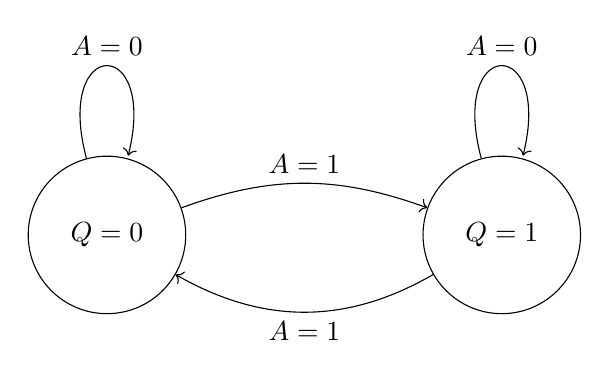
\begin{tikzpicture}[node distance=3cm]
    \node[circle,draw,minimum width=2cm](s0){$Q=0$};
    \node[circle,draw,minimum width=2cm](s1)[right=of s0]{$Q=1$};
    \path(s0)edge[loop above]node[above]{$A=0$} (s0);
    \path(s1)edge[loop above]node[above]{$A=0$}(s1);
    \path(s0)[->]edge[bend right=-20]node[above]{$A=1$}(s1);
    \path(s1)[->]edge[bend left=30]node[below]{$A=1$}(s0);
\end{tikzpicture}

        \end{figure}
\pagebreak
\item{(B)}
        \begin{figure}[h]
         	\centering
	        \begin{tikzpicture}[node distance=3cm]
    \node[circle,draw,minimum width=2cm](s0){$Q=0$};
    \node[circle,draw,minimum width=2cm](s1)[right=of s0]{$Q=1$};
    \path(s0)edge[loop above]node[above]{$A=0$} (s0);
    \path(s0)[->]edge[bend right=-20]node[above]{$A=1$}(s1);
    \path(s0)[->]edge[bend left=-50]node[above]{$A=0$}(s0);
    \path(s1)[->]edge[bend left=30]node[below]{$A=1$}(s0);
     \end{tikzpicture}

        \end{figure}
\item{(C)}
	\begin{figure}[h]
		\centering
		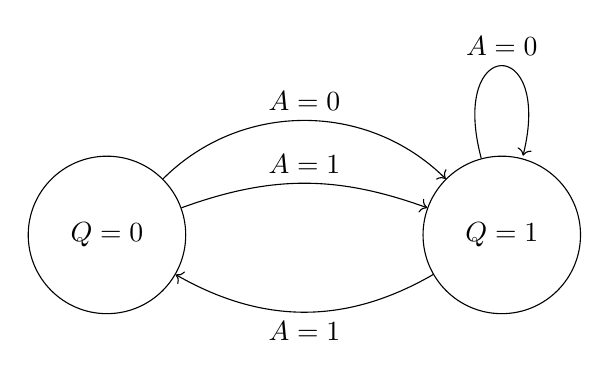
\begin{tikzpicture}[node distance=3cm]
    \node[circle,draw,minimum width=2cm](s0){$Q=0$};
    \node[circle,draw,minimum width=2cm](s1)[right=of s0]{$Q=1$};
    \path(s1)edge[loop above]node[above]{$A=0$} (s1);
    \path(s0)[->]edge[bend right=-20]node[above]{$A=1$}(s1);
    \path(s0)[->]edge[bend right=-45]node[above]{$A=0$}(s1);
    \path(s1)[->]edge[bend left=30]node[below]{$A=1$}(s0);
     \end{tikzpicture}

	\end{figure}
\item{(D)}
	\begin{figure}[h]
		\centering
		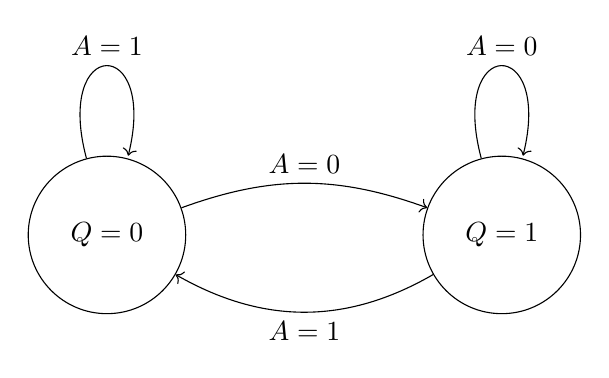
\begin{tikzpicture}[node distance=3cm]
    \node[circle,draw,minimum width=2cm](s0){$Q=0$};
    \node[circle,draw,minimum width=2cm](s1)[right=of s0]{$Q=1$};
    \path(s0)edge[loop above]node[above]{$A=1$} (s0);
    \path(s1)edge[loop above]node[above]{$A=0$}(s1);
    \path(s0)[->]edge[bend right=-20]node[above]{$A=0$}(s1);
    \path(s1)[->]edge[bend left=30]node[below]{$A=1$}(s0);
     \end{tikzpicture}

	\end{figure}
\end{enumerate}
\pagebreak
\section{Components}
 \begin{table}[h]
  \centering
   \begin{tabular}{|c|c|c|}
   \hline
   \textbf{Component}& \textbf{Values} & \textbf{Quantity}\\
\hline
ArduinoUNO &  & 1 \\  
\hline
JumperWires& M-M & 10 \\ 
\hline
Breadboard &  & 1 \\
\hline
LED & &1 \\
\hline
Resistor &220ohms & 1\\
\hline
   \end{tabular}
   \end{table}
\section{Reduction of logical circuit}
The output of 2:1 mux is P.\\
Now , $P=AQ+A'Q'$\\
$D=(Q.P)'$\\
$D=(Q(AQ+A'Q'))'$\\
 $D=(A(Q.Q)+(A'Q'Q))'$
 $D=(AQ)'$\\
 The equation after reducing the logical circuit is:\\
 $D=(AQ)'$\\

 \section{Truth table}
 \begin{table}[h]
  \centering
   \begin{tabular}{|c|c|c|}
   \hline
   Q & A & Q'\\
   \hline
   0 & 0 & 1\\
   \hline
   1 & 0 & 0\\
   \hline
   1 & 1 & 0\\
   \hline
   0 & 1 & 1\\
   \hline
   \end{tabular}
   \end{table}
\section{Next stages}
\begin{figure}[h]
	\centering
	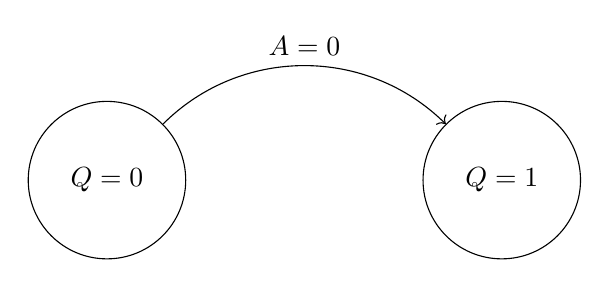
\begin{tikzpicture}[node distance=3cm]
    \node[circle,draw,minimum width=2cm](s0){$Q=0$};
    \node[circle,draw,minimum width=2cm](s1)[right=of s0]{$Q=1$};
    \path(s0)[->]edge[bend right=-45]node[above]{$A=0$}(s1);
\end{tikzpicture}

	\caption{Stage 1}
\end{figure}
\pagebreak
\begin{figure}[h]
        \centering                                  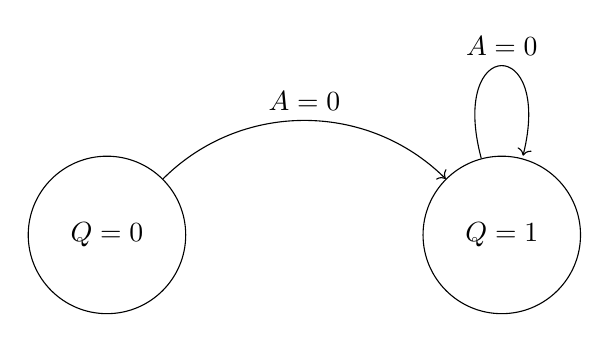
\begin{tikzpicture}[node distance=3cm]
    \node[circle,draw,minimum width=2cm](s0){$Q=0$};
    \node[circle,draw,minimum width=2cm](s1)[right=of s0]{$Q=1$};
    \path(s1)edge[loop above]node[above]{$A=0$} (s1);
    \path(s0)[->]edge[bend right=-45]node[above]{$A=0$}(s1);
\end{tikzpicture}

        \caption{Stage 2}
\end{figure}
\begin{figure}[h]
        \centering
	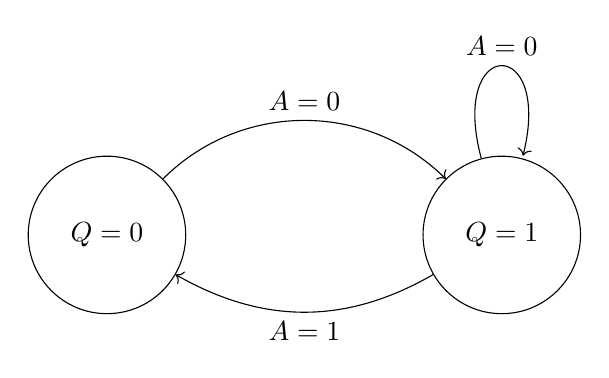
\begin{tikzpicture}[node distance=3cm]
    \node[circle,draw,minimum width=2cm](s0){$Q=0$};
    \node[circle,draw,minimum width=2cm](s1)[right=of s0]{$Q=1$};
    \path(s1)edge[loop above]node[above]{$A=0$} (s1);
    \path(s0)[->]edge[bend right=-45]node[above]{$A=0$}(s1);
    \path(s1)[->]edge[bend left=30]node[below]{$A=1$}(s0);
\end{tikzpicture}

	\caption{Stage 3}
\end{figure}
\pagebreak
\begin{figure}[h]
        \centering                                  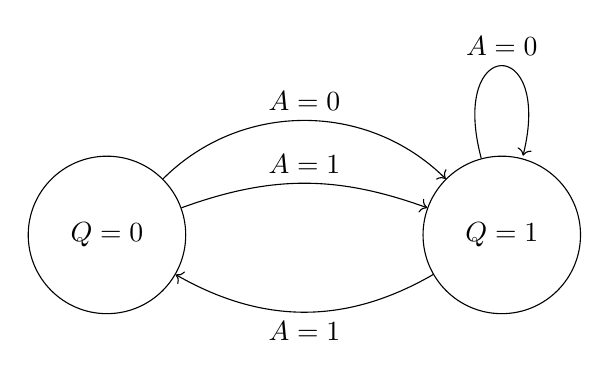
\begin{tikzpicture}[node distance=3cm]
    \node[circle,draw,minimum width=2cm](s0){$Q=0$};
    \node[circle,draw,minimum width=2cm](s1)[right=of s0]{$Q=1$};
    \path(s1)edge[loop above]node[above]{$A=0$} (s1);
    \path(s0)[->]edge[bend right=-20]node[above]{$A=1$}(s1);
    \path(s0)[->]edge[bend right=-45]node[above]{$A=0$}(s1);
    \path(s1)[->]edge[bend left=30]node[below]{$A=1$}(s0);
\end{tikzpicture}

        \caption{Stage 4}
\end{figure} 

\section{implementation}
\begin{table}[h]
  \centering
  \begin{tabular}{|c|c|c|}
\hline
\textbf{Arduino pin} & \textbf{INPUT} & \textbf{OUTPUT}\\
\hline
2 & Q &\\
\hline
3 & A &\\
\hline
8 & & D\\
\hline
  \end{tabular}
\end{table}
\section{Procedure}
   1. Connect the circuit as per the above table.\\
   2. Connect the Output pin D to the LED.\\
   3. Connect the other end of the LED to the Ground terminal.\\
   4. Connect inputs to Vcc for logic 1,ground for logic 0.\\
   5. Execute the circuits using the below code.\\
   \begin{table}[h]
	   \centering
	   \begin{tabular}{|c|}
	   \hline
	   https://github.com/pavangoudmanchanpally/ec392019/blob/main/code/ec392019.cpp\\
	   \hline
	   \end{tabular}
   \end{table}\\
   6. Change the values of Q and A in the code and verify the Truth table .\\

 

\end{document}

